8. $f(x)=\cfrac{\cos\left(\cfrac{3x}{2}
ight)-\cos\left(\cfrac{x}{2}
ight)}
{\sqrt{\cos^2(x)+\sin^2(x)-2\cos(2x)+1}}+\left|\sin\left(\cfrac{x}{2}
ight)
ight|=
\cfrac{-2\sin(x)\sin\left(\cfrac{x}{2}
ight)}{\sqrt{2(1-\cos(2x))}}+\left|\sin\left(\cfrac{x}{2}
ight)
ight|=$\\$
\cfrac{-2\sin(x)\sin\left(\cfrac{x}{2}
ight)}{\sqrt{4\sin^2(x)}}+\left|\sin\left(\cfrac{x}{2}
ight)
ight|=
\cfrac{-\sin(x)\sin\left(\cfrac{x}{2}
ight)}{|\sin(x)|}+\left|\sin\left(\cfrac{x}{2}
ight)
ight|.$
Таким образом, при $x\in\left(-\pi;\pi
ight)+2\pi k\ (k\in \mathbb{Z})$ имеем $f(x)=0,$ а при $x\in\left(\pi;3\pi
ight)+2\pi k\ (k\in \mathbb{Z})$ имеем $f(x)=2\sin\left(\cfrac{x}{2}
ight)$ за исключением точек $x=\pi k\ (k\in \mathbb{Z}),$ которые являются выколотыми.
$$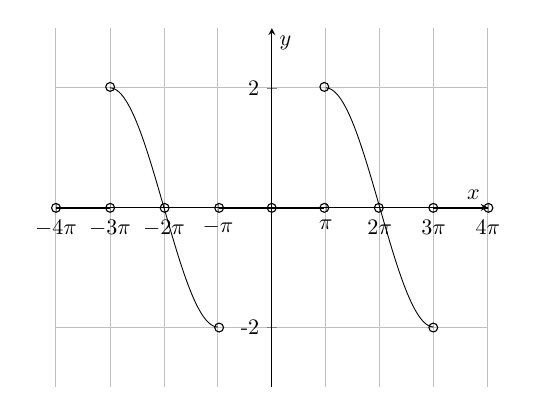
\begin{tikzpicture}[scale=0.8]
\tikzset{line02/.style={line width =0.8pt}}
\begin{axis}[
    axis lines = middle,
    grid=major,
    legend pos={south west},
    xlabel = {$x$},
    ylabel = {$y$},
    ymin=-3,
    ymax=3,
    xtick={-12.57,-9.42,-6.28,-3.14, 3.14, 6.28, 9.42, 12.57},
    xticklabels={$-4\pi$, $-3\pi$, $-2\pi$, $-\pi$, $\pi$, $2\pi$, $3\pi$, $4\pi$},
    ytick={2,-2},
    yticklabels={2,-2}          ]
	\addplot[domain=pi:3*pi, samples=100, color=black] {2*sin(deg(x/2))};
    \addplot[domain=-3*pi:-pi, samples=100, color=black] {2*sin(deg(x/2))};
    \addplot[domain=3*pi:4*pi, samples=100, color=black] {0};
    \addplot[domain=-4*pi:-3*pi, samples=100, color=black] {0};
%\addplot[domain=-3.1:2.5, samples=100, color=red] {70*abs(1-2*abs(abs(x)-2))-10*x^2+10*x-70};
	%\addlegendentry{$\text{Рис. 1}$};
\end{axis}
%\draw[line02] (0.9,2.84) -- (2.55,2.84);
%\draw[line02] (4.3,2.84) -- (5.95,2.84);
\draw[line02] (0,2.84) -- (0.86,2.84);
\draw[line02] (2.59,2.84) -- (4.26,2.84);
\draw[line02] (5.99,2.84) -- (6.865,2.84);
\draw (0.86,2.84) circle (2pt);
\draw (2.59,2.84) circle (2pt);
\draw (0.86,4.76) circle (2pt);
\draw (2.59,0.94) circle (2pt);
\draw (1.725,2.84) circle (2pt);
\draw (0,2.84) circle (2pt);

\draw (3.425,2.84) circle (2pt);

\draw (4.26,4.76) circle (2pt);
\draw (5.99,2.84) circle (2pt);
\draw (4.26,2.84) circle (2pt);
\draw (5.99,0.94) circle (2pt);
\draw (5.125,2.84) circle (2pt);

\draw (6.865,2.84) circle (2pt);
\end{tikzpicture}$$
